% Shared standalone design for the editable figure reconstructions.
\documentclass[tikz,border=5pt,10pt]{standalone}
\usepackage[T1]{fontenc}
\usepackage[utf8]{inputenc}
\usepackage{newpxtext,newpxmath}
\usepackage[scaled=.94]{sourcesanspro}
\usepackage{pgfplots}
\pgfplotsset{compat=1.18}
\usetikzlibrary{arrows.meta,calc,positioning,decorations.pathreplacing,
  decorations.markings,patterns,matrix,shapes.geometric,fit,backgrounds,
  intersections,angles,quotes}
\definecolor{ink}{HTML}{203746}
\definecolor{accent}{HTML}{146C78}
\definecolor{muted}{HTML}{667780}
\definecolor{signalred}{HTML}{B94B44}
\color{ink}
\tikzset{>=Latex,line width=.8pt,
  every node/.style={font=\small},
  axis/.style={->,draw=muted,line width=.5pt},
  guide/.style={draw=muted,dashed,line width=.45pt},
  curve/.style={draw=accent,line width=1pt},
  marker/.style={circle,fill=accent,inner sep=1.5pt},
  labelbox/.style={fill=white,inner sep=2pt}}

\begin{document}
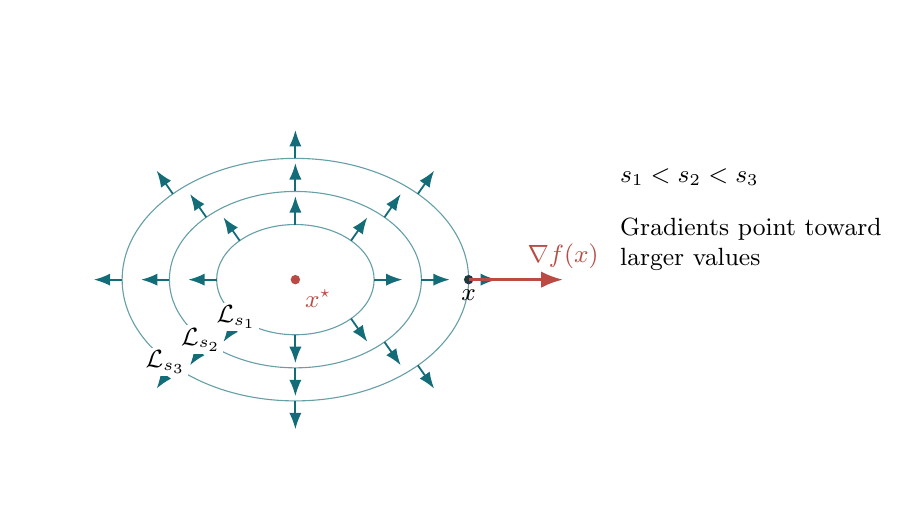
\begin{tikzpicture}
\path[use as bounding box] (-3.4,-2.8) rectangle (7.6,3.2);\draw[accent!65] (0,0) ellipse (1 and 0.7);
\draw[->,accent,line width=.65pt] (1.0000,0.0000)--(1.3600,0.0000);
\draw[->,accent,line width=.65pt] (0.7071,0.4950)--(0.9136,0.7899);
\draw[->,accent,line width=.65pt] (0.0000,0.7000)--(0.0000,1.0600);
\draw[->,accent,line width=.65pt] (-0.7071,0.4950)--(-0.9136,0.7899);
\draw[->,accent,line width=.65pt] (-1.0000,0.0000)--(-1.3600,0.0000);
\draw[->,accent,line width=.65pt] (-0.7071,-0.4950)--(-0.9136,-0.7899);
\draw[->,accent,line width=.65pt] (-0.0000,-0.7000)--(-0.0000,-1.0600);
\draw[->,accent,line width=.65pt] (0.7071,-0.4950)--(0.9136,-0.7899);
\node[fill=white,inner sep=1pt] at (-0.75,-0.476) {$\mathcal L_{s_1}$};
\draw[accent!65] (0,0) ellipse (1.6 and 1.1199999999999999);
\draw[->,accent,line width=.65pt] (1.6000,0.0000)--(1.9600,0.0000);
\draw[->,accent,line width=.65pt] (1.1314,0.7920)--(1.3378,1.0869);
\draw[->,accent,line width=.65pt] (0.0000,1.1200)--(0.0000,1.4800);
\draw[->,accent,line width=.65pt] (-1.1314,0.7920)--(-1.3378,1.0869);
\draw[->,accent,line width=.65pt] (-1.6000,0.0000)--(-1.9600,0.0000);
\draw[->,accent,line width=.65pt] (-1.1314,-0.7920)--(-1.3378,-1.0869);
\draw[->,accent,line width=.65pt] (-0.0000,-1.1200)--(-0.0000,-1.4800);
\draw[->,accent,line width=.65pt] (1.1314,-0.7920)--(1.3378,-1.0869);
\node[fill=white,inner sep=1pt] at (-1.2000000000000002,-0.7615999999999999) {$\mathcal L_{s_2}$};
\draw[accent!65] (0,0) ellipse (2.2 and 1.54);
\draw[->,accent,line width=.65pt] (2.2000,0.0000)--(2.5600,0.0000);
\draw[->,accent,line width=.65pt] (1.5556,1.0889)--(1.7621,1.3839);
\draw[->,accent,line width=.65pt] (0.0000,1.5400)--(0.0000,1.9000);
\draw[->,accent,line width=.65pt] (-1.5556,1.0889)--(-1.7621,1.3839);
\draw[->,accent,line width=.65pt] (-2.2000,0.0000)--(-2.5600,0.0000);
\draw[->,accent,line width=.65pt] (-1.5556,-1.0889)--(-1.7621,-1.3839);
\draw[->,accent,line width=.65pt] (-0.0000,-1.5400)--(-0.0000,-1.9000);
\draw[->,accent,line width=.65pt] (1.5556,-1.0889)--(1.7621,-1.3839);
\node[fill=white,inner sep=1pt] at (-1.6500000000000001,-1.0472000000000001) {$\mathcal L_{s_3}$};
\fill[signalred] (0,0) circle (1.7pt) node[below right] {$x^\star$};
\coordinate (X) at (2.2,0);\fill[ink] (X) circle (1.7pt);\draw[->,signalred,line width=1.1pt] (X)--(3.4,0) node[above] {$\nabla f(x)$};\node[below] at (2.2,0) {$x$};
\node[anchor=west] at (4,1.3) {$s_1<s_2<s_3$};\node[anchor=west,align=left] at (4,.45) {Gradients point toward\\larger values};
\end{tikzpicture}
\end{document}
